\documentclass[a4paper, 12pt]{article}
\usepackage[english, russian]{babel}
\usepackage{svg}
\usepackage[T2A]{fontenc}
\usepackage[utf8]{inputenc}
\usepackage{ stmaryrd }
\usepackage{ dsfont, amsmath, amsfonts, amssymb, amsthm, mathtools }
\theoremstyle{plain}
\usepackage{listings}
\usepackage{xcolor}
\newtheorem{theorem}{Теорема}
\newtheorem{lemma}{Лемма}
\newtheorem{definition}{Определение}
\usepackage[english, russian]{babel}
\usepackage[T2A]{fontenc}
\usepackage[utf8]{inputenc}
\usepackage{amssymb}
\usepackage{amsmath}
\usepackage{amsfonts}
\usepackage{geometry}
\geometry{top=15mm}
\geometry{bottom=15mm}
\geometry{left=15mm}
\geometry{right=15mm}
\linespread{1.3}
\usepackage{graphicx}
\usepackage{graphicx}
\usepackage{setspace}
\usepackage{amsmath}
\usepackage{tikz}
\usetikzlibrary{graphs}
\usepackage{amscd}
\usepackage[all]{xy}
\definecolor{codegreen}{rgb}{0,0.6,0}
\definecolor{codegray}{rgb}{0.5,0.5,0.5}
\definecolor{codepurple}{rgb}{0.58,0,0.82}
\definecolor{backcolour}{rgb}{0.95,0.95,0.92}
\lstdefinestyle{mystyle}{
	backgroundcolor=\color{backcolour},   
	commentstyle=\color{codegreen},
	keywordstyle=\color{magenta},
	numberstyle=\tiny\color{codegray},
	stringstyle=\color{codepurple},
	basicstyle=\ttfamily\footnotesize,
	breakatwhitespace=false,         
	breaklines=true,                 
	captionpos=b,                    
	keepspaces=true,                 
	numbers=left,                    
	numbersep=5pt,                  
	showspaces=false,                
	showstringspaces=false,
	showtabs=false,                  
	tabsize=2
}

\lstset{style=mystyle}

\begin{document}
	\setcounter{page}{1}
	
	\begin{center} 
		\textbf{Правительство Российской Федерации}
		\\ \textbf{Федеральное государственное автономное образовательное учреждение}
		\\ \textbf{высшего профессионального образования}
		\\ \textbf{«Национальный исследовательский университет»}
		\\ \textbf{«Высшая школа экономики»}
		\\ \textbf{Нижегородский кампус}
		\vspace{3cm}
		\\ Факультет математики, информатики и компьютерных наук
		\\ Кафедра фундаментальной математики
		\vspace{3cm}
		\\ \large\textbf{КУРСОВАЯ РАБОТА}
		\vspace{0.3cm}
		\\ \large\textbf{ГЕНЕРАЦИЯ 3D-ИЗОБРАЖЕНИЙ ДИСКРЕТНЫХ ДИНАМИЧЕСКИХ СИСТЕМ, ЗАДАННЫХ НА ПОВЕРХНОСТЯХ, ИЗ ТРЁХЦВЕТНЫХ ГРАФОВ}
	\end{center}
	
	\vspace{3cm}\hspace{8cm} Выполнил: 
	\par \hspace{8cm} Студент 2 курса группы 22 ФМ 
	\par \hspace{8cm} Турсунов Данил Вячеславович
	\par \vspace{0.8cm} \hspace{8cm} Научный руководитель:
	\par \hspace{8cm} Баринова Марина Константиновна
	\begin{center} 
		\vspace{4cm} Нижний Новгород
		\par Май 2024 г.
	\end{center}
	\newpage
	
	\tableofcontents
	\newpage

	\section{Вступление}
	\subsection{Цели и задачи работы}
		\hspace{0.5 cm} Основной целью работы является создание приложения на языках C++ и Python с применением библиотеки Manim. Суть приложения заключается в генерации 3D-изображений градиентно-подобных каскадов, заданных на сфере, из соответствующих им трёхцветных графов, заранее проверенных программой на корректность. Алгоритмическая часть приложения написана на C++, так как этот язык в разы быстрее чем язык Python, а на языке Python написана визуальная составляющая программы, так как язык содержит множество удобных для этого библиотек.
		\par Помимо этого поставлены следующие подзадачи:
		\par 1) Разобраться в связи градиентно-подобных каскадов и трёхцветных графов;
		\par 2) Научиться писать Unit-тесты на языке C++, необходимые для стабильной работы программы при её изменении в дальнейшем;
		\par 3) Придумать алгоритм генерации трёхцветных графов с заданными параметрами: число Эйлера и число сёдел динамической системы.
	\subsection{Актуальность работы}
		\hspace{0.5 cm} Программа, написанная в результате работы, будет полезна начинающим научным сотрудникам или обычным студентам, желающим разобраться в градиентно-подобных каскадах на сфере, так как она поможет им быстрее визуализировать эти динамические системы. Помимо этого, отдельные функции из алгоритмический части могут быть полезны другим исследователям трёхцветных графов в написании программ в дальнейшем.
	\newpage
	
	\section{Теоретическая часть}
	\subsection{Описание}
	\hspace{0.5 cm} В этой главе будут представлены: введение в теорию графов, алгоритм построения трёхцветного графа по градиентно-подобному каскаду на поверхности, свойства и определение трёхцветного графа, сформулированные в теоремах и определениях.
	\subsection{Введение в теорию графов и построение трёхцветного графа по каскаду}
	\hspace{0.5 cm} Начнём введение в теоретическую часть с определения диффеоморфизма Морса-Смейа и алгоритма построения трёхцветного графа, заданного на поверхности и, в частности, на сфере.
	\begin{definition} (Диффеоморфизм Морса-Смейла) $\\$
		Диффеоморфизм $f: M^n \shortrightarrow M^n$, заданный на гладком замкнутом n-многообразии, называется диффеоморфизмом Морса-Смейла, если:
		\par 1) неблуждающее множество $\Omega_f$ гиперболично и конечно (т.е. состоит из конечного чила периодических точек, для которых модули собственных значений матрицы Якоби не равны единице);
		\par 2) для любых периодических точек p, q устойчивое многообразие $W^s_p$ и неустойчивое многообразие $W^u_q$ либо не пересекаются, либо трансверсальны в каждой точке пересечения.
	\end{definition}
	Пусть $f: M^n \shortrightarrow M^n$ - диффеоморфизм Морса-Смейла, тогда периодические точки называются источниками, если неустойчивое многообразие $W^u_q$ имеет размерность $n$, стоками, если  размерность равна $0$, и сёдлами при остальных значениях размерности.
	\par Далее скажем, что для любой периодической точки $p$ диффеоморфизма $f$ компоненты связности $W^s_p (p)$ и $(W^u_p (p))$ называются её устойчивыми или неустойчивыми сепаратрисами соответственно.
	\par Введём более узкое определение: рассмотрим класс диффеоморфизмов на поверхности $M^2$, тогда диффеоморфизм Морса-Смейла называется градиентно-подобным, если $W^s_p \cap W^u_p = \o$ для любых различных седловых точек $p,q$.
	\par В дальнейшем в работе будут рассматриваться исключительно граентно-подобные диффеоморфизмы, заданные на поверхности $M^2$. Класс градиетно-подобных диффеоморфизмов, заданных на поверхности $M^2$, обозначим $G$.
	\par Удалим из поверхности $M^2$ замыкание объединения устойчивых и неустойчивых многообразий седловых точек $f$ и получим множество $M'$.
	$M'$ является объединением ячеек, гомеоморфных открытому двумерному диску, граница которых имеет один из 3-х видов, показанных на рис. 1.
	\begin{figure}[h!]
		\centering
		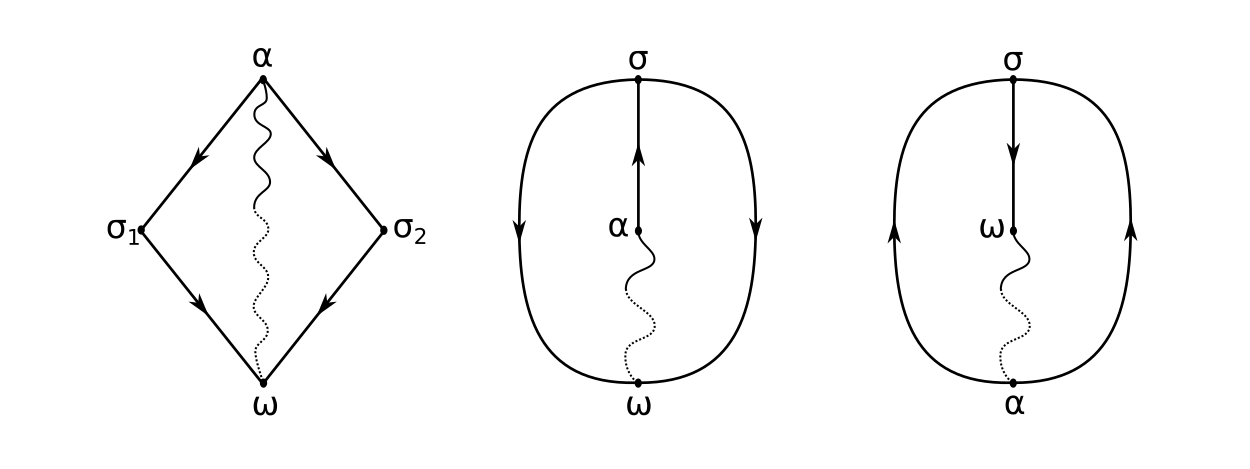
\includegraphics[width=\textwidth]{Cells.png}
		\caption{Возможные ячейки множества $M'$. \label{overflow}}
	\end{figure}
	\par Пусть $A$ - ячейка из $M'$, $\alpha$ и $\omega$ - источник и сток, входящие в её границу. Кривую $\tau\in A$, началом и концом которой являеются $\alpha$ и $\omega$, будем называть $t-$кривой. Через $T$ обозначим множество $t-$кривых, взятых по одной из каждой ячейки. $\\$
	\par Разобьём каждую ячейку этой кривой на 2 области, компоненты связности $M_\Delta = M' \textbackslash T$ назовём треугольными областями. В границу каждой треугольной области входят 3 периодические точки: источник, сток и седло, а также устойчивая сепаратриса, неусточивая сепаратриса и кривая $\tau$. В дальнейшем будем называть их $s-$кривой, $u-$кривой и $t-$кривой соответственно. Замыкание каждой из этих кривых будем называть стороной треугольной области. Скажем, что сторона является общей стороной для двух треугольных областей, если она принадлежит замыканиям этих треугольных областей.
	\par Для дальнейшего введения в теорию трёхцветных графов потребуется ввести некоторые определения из теории графов.
	\begin{definition} (Конечный граф) $\\$
		Конечным графом называется упорядоченная пара (B,E), для которой выполнены следующие условия:
		\par 1) B - непустое конечное множество вершин;
		\par 2) E - множество пар вершин, называемых рёбрами.
	\end{definition}
	\begin{definition} (Инцидентность) $\\$
		Если граф содержит ребро e = (a,b), то каждую из вершин a, b называют инцидентной ребру e и говорят, что вершины a и b соединены ребром e.
	\end{definition}
	\begin{definition} (Путь в графе) $\\$
		Путём в графе называют конечную последовательность его вершин и рёбер вида: $b_0, (b_0, b_1), b_1, \dots, b_{i-1}, (b_{i-1}, b_{i}), b_{i}, \dots, b_{k-1}, (b_{k-1}, b_{k}), b_{k}, k >= 1$. Число k называется длиной пути, оно совпадает с числом входящих в него рёбер.
	\end{definition}
	\begin{definition} (Цикл в графе) $\\$
		Циклом длины $k \in \mathds{N}$ в графе называют конечное подмножество его вершин и рёбер вида \{$b_0, (b_0, b_1), b_1, \dots, b_{i-1}, (b_{i-1}, b_{i}), b_{i}, \dots, b_{k-1}, (b_{k-1}, b_{0})$\}. Простым циклом называют цикл, у которого все вершины и рёбра попарно различны.
	\end{definition}
	\begin{definition} (Связность графа) $\\$
		Граф называют связным, если любые две его вершины можно соединить путём.
	\end{definition}
	С учётом имеющихся у нас вводных, введём определение трёхцветного графа, а также сформулируем некоторые теоремы.
	\begin{definition} (Трёхцветный граф) $\\$
		Граф T называется трёхцветным графом, если:
		\par 1) множество рёбер графа T является объединением трёх подмножеств, каждое из которых состоит из трёх рёбер одного и того же определенного цвета (цвета рёбер из разных подмножеств не совпадают, будем обозначать эти цвета буквами s, t, u, а рёбра для краткости будем называть s-, t-, u-рёбрами);
		\par 2) каждая вершина графа T инцидентна в точности трём рёбрам различных цветов;
		\par 3) граф не содержит циклов длины 1.
	\end{definition}
	\begin{definition} (Двухцветный цикл) $\\$
		Простой цикл трёхцветного графа T назовём двухцветным su-, tu- или st-циклом, если он содержит рёбра в точности двух цветов s и u, t и u, s и t соответственно.
	\end{definition}
	 Непосредственно из определения трёхцветного графа следует, что длина любого двухцветного цикла является чётным числом (так как цвета рёбер строго чередуются), а отношение на множестве вершин, состоящее в принадлежности двухцветному циклу определённого типа, является отношением эквивалентности, то есть каждая отдельно взятая вершина лежит в точности в одном  $su-$, одном $tu-$ и одном $st-$цикле.
	\begin{definition} (Построение трёхцветного графа по диффеоморфизму) $\\$
		Построим трёхцветный граф $T_f$, соответствующий диффеоморфизму $f \in G$, следующим образом:
		\par 1) вершины графа $T_f$ взаимно однозначно соответствуют треугольным областям множества $\Delta$;
		\par 2) две вершины графа инцидентны ребру цвета s, t, u, если соответствующие этим вершинам треугольные области имеют общую s-, t- или u-кривую .
	\end{definition}
	Отметим, что построенный граф $T_f$ полностью удовлетворяет определению трёхцветного графа.
	\begin{definition} (Допустимость трёхцветного графа) $\\$
		Трёхцветный граф (T,P) назовём допустимым, если он обладает следующими свойствами:
		\par 1) граф T связен;
		\par 2) длина любого su-цикла графа T равна 4;
		\par 3) автоморфизм P является периодическим.
	\end{definition}
	Отметим, что трёхцветный граф, построенный по градиентно-подобному каскаду на поверхности, является допустимым. Следующие теоремы сформулированы для трёхцветных графов, оснащённых автоморфизмом, однако, во избежание излишей громоздкости теоретической части, данная часть повествования была опущена в курсовой работе.
	\begin{theorem} (Топологическая сопряжённость диффеоморфизмов) $\\$
	Для того чтобы диффеоморфизмы f, f' из класса G были топологически сопряжены, необходимо и достаточно, чтобы их графы ($T_f, P_f$) и ($T_{f'}, P_{f'}$) были изоморфны.
	\end{theorem}
	\begin{theorem} (Свойства допустимого трёхцветного графа) $\\$
		Пусть (T,P) - допустимый трёхцветный граф. Тогда существует диффеоморфизм $f:M^2 \shortrightarrow M^2$ из класса G, граф ($T_f, P_f$) которого изоморфен графу (T,P). При этом:
		\par 1) эйлерова характеристика поверхности $M^2$ вычисляется по формуле $X(M^2) = v_0 - v_1 + v_2$, где $v_0, v_1, v_2$ - число всех tu-, su-, st-циклов графа T соответственно;
		\par 2) поверхность $M^2$ ориентируема тогда и только тогда, когда все циклы графа T имеют чётную длину.
	\end{theorem}
	\newpage
	
	\section{Алгоритмическая часть}
	\subsection{Структура программы}
	\hspace{0.5 cm} Программа состоит из 2 частей: алгоритмической и графической, каждая из частей запускается отдельно и независимо друг от друга. Изначально запускается алгоритмическая часть на языке C++, туда вводится корректный трёхцветный граф, программа его обрабатывает и выдаёт в отдельном файле координаты сепаратрис. Далее запускается графическая часть программы, написанная на языке Python. Она считывает координаты из файла и генерирует по заданным координатам конца и начала сепаратрис 3D-изображение, а затем, после рендеринга в библиотеке Manim, показывает её пользователю.
	\subsection{Проверка введённого трёхцветного графа на корректность}
	\hspace{0.5 cm} Проверяет граф на корректность функция $is\textunderscore acceptable$, которая принимает на вход заданный граф и возвращает булевое значение: True, если граф является корректным (допустимым) трёхцветным графом, и False, если граф таковым не является.
	\par Согласно определению 10 граф называется корректым трёхцветным графом, если:
	\par 1) граф является трёхцветным, то есть попадает под определение трёхцветности;
	\par 2) граф является связным;
	\par 3) все SU-циклы в графе имеют длину равную четырём.
	\par Функция для проверки пункта 1 вызывает функцию $is \textunderscore 3 \textunderscore colored \textunderscore and \textunderscore non \textunderscore oriented$, которая действует следующим образом: функция циклом проходит по вершинам графа, для каждой вершины проверяет, действительно ли из неё выходит только 3 ребра, причем эти рёбра должны быть разных цветов: $u$, $s$ и $t$. Параллельно с этим в этом же цикле проверяется то, что граф является неориентируемым, а также то, что граф не содержит петель, то есть циклов длины 1. Если хотя бы одно из условий не выполняется, функция возвращает False, в противном случае она возращает True.
	\par Для проверки пункта 2 функция вызывает функцию $is \textunderscore connected$, которая считает расстояния от вершины с порядковым номером 0 до остальных вершин при помощи функции $bfs$. Здесь под расстоянием имеется в виду длина кратчайшего пути между 2 вершинами. Если не существует пути, соединяющего 2 вершины, расстояние считается равным $inf$. Если хотя бы одно расстояние окажется равным $inf$, то граф не связен и функция вернёт значение False, а в противном случае граф является связным и функция возвращает значение True.
	\par Функция $bfs$ принимает на вход начальную вершину (в данном случае это вершина с номером 0) и сам граф и работает по алгоритму $breadth-first~search$, что можно перевести как <<поиск в ширину>>. Алгоритм работает с применением структуры данных <<очередь>>. Принцип работы этой структуры данных объясняется фразой: <<Первый зашёл - последний вышел.>>. Алгоритм работает следующим образом: создаётся вектор, стуктура данных для хранения данных в C++, содержащий известные расстояния от начальной вершины до остальных, изначально заполнен $inf$, кроме начальной, так как расстояние от начальной до начальной вершины равно 0, и очередь, состоящая только из начальной вершины, далее запускается цикл, он работает до тех пор, пока очередь не опустеет. В каждой итерации цикл делает первую вершину из очереди текущей и проходит по всем соседним вершинам текущей (то есть тем, кто соединён с ней ребром), и, если известное расстояние до соседа больше суммы расстояния до текущей и единицы (она появляется за счёт ребра, которое их соединяет), то минимальное известное расстояние обновляется, а вершина-сосед кладётся в очередь. Функция возвращает вектор расстояний до каждой из вершин.
	\par Для проверки пункта 3 функция вызывает функцию $find \textunderscore cycles$ с переданными в неё графом, литералами <<s>> и <<u>>, которые отвечают за то, какого цвета циклы надо найти. Функция $find \textunderscore cycles$ возвращает вектор, состоящий из циклов, каждый цикл представляет собой последовательность номеров вершин цикла, так же последовательно соединённых между собой в самом цикле. Эта функция в процессе своего исполнения использует факт, который вытекает из определений 7 и 8 про то, что каждая отдельно взятая вершина лежит только в одном $su-$, одном $tu-$ и одном $st-$цикле, поэтому каждый цикл по отдельности ищется функцией $find \textunderscore cycle$ достаточно тривиальным алгоритмом, который просто идёт по циклу из начальной вершины, пока снова не встретит начальную вершину. Далее функция $is\textunderscore acceptable$ проверяет, имеют ли все SU-циклы в графе длину 4.
	\par Если все условия выполнены, функция $is\textunderscore acceptable$ возвращает True, в противном случае возвращает False.
	\subsection{Проверка поверхности на ориентируемость}
	\hspace{0.5 cm} Для построения алгоритма, проверяющего поверхность, на которой задан градиентно-подобный каскад, по трёхцветному графу, потребуется пункт 2 теоремы 2, который гласит о том, что поверхности ориентируема тогда и только тогда, когда все циклы графа имеют чётную длину.
	\par Сделать вывод о четной длине всех циклов графа можно найдя хотя бы один цикл нечётной длины. Для нахождения такого цикла потребуется небольшой экскурс в теорию, связанную с базой циклов и алгоритмом её нахождения.
	\par Базой циклов неориентированного графа является такой набор циклов, путём соединения или вычитания которых могут получиться все остальные циклы. Для нахождения базы циклов необходимо построить из графа так называемое <<переплетающееся дерево>> (spanning tree), то есть просто выбрать какую-нибудь вершину за корень дерева, а потом идти по нему уже упомянутым выше алгоритмом поиска в ширину из корневой вершины, при этом вместо поиска расстояний отмечать посещённые вершины, если вершина-сосед не посещена, то ребро, связывающее текущую вершину с ней, добавлять в <<переплетающееся дерево>>, а далее, путём добавления по одному в дерево рёбер изначального графа, которые в дерево не попали, по одному найти все циклы. Эти циклы и будут составлять базу циклов в графе. Очевидно, что при вычитании или сложении циклов четной длины получится цикл чётной длины, то есть на чётность достаточно проверить всего лишь циклы из базы циклов.
	\par Алгоритм, находящий <<переплетающееся дерево>> и сразу проверяющий циклы базы циклов на чётную длину, реализован в функции $is \textunderscore oriented \textunderscore surface$, которая возвращает True, если поверхность ориентируема, и False, если поверхность неориентируема.
	\begin{figure}[h!]
		\centering
		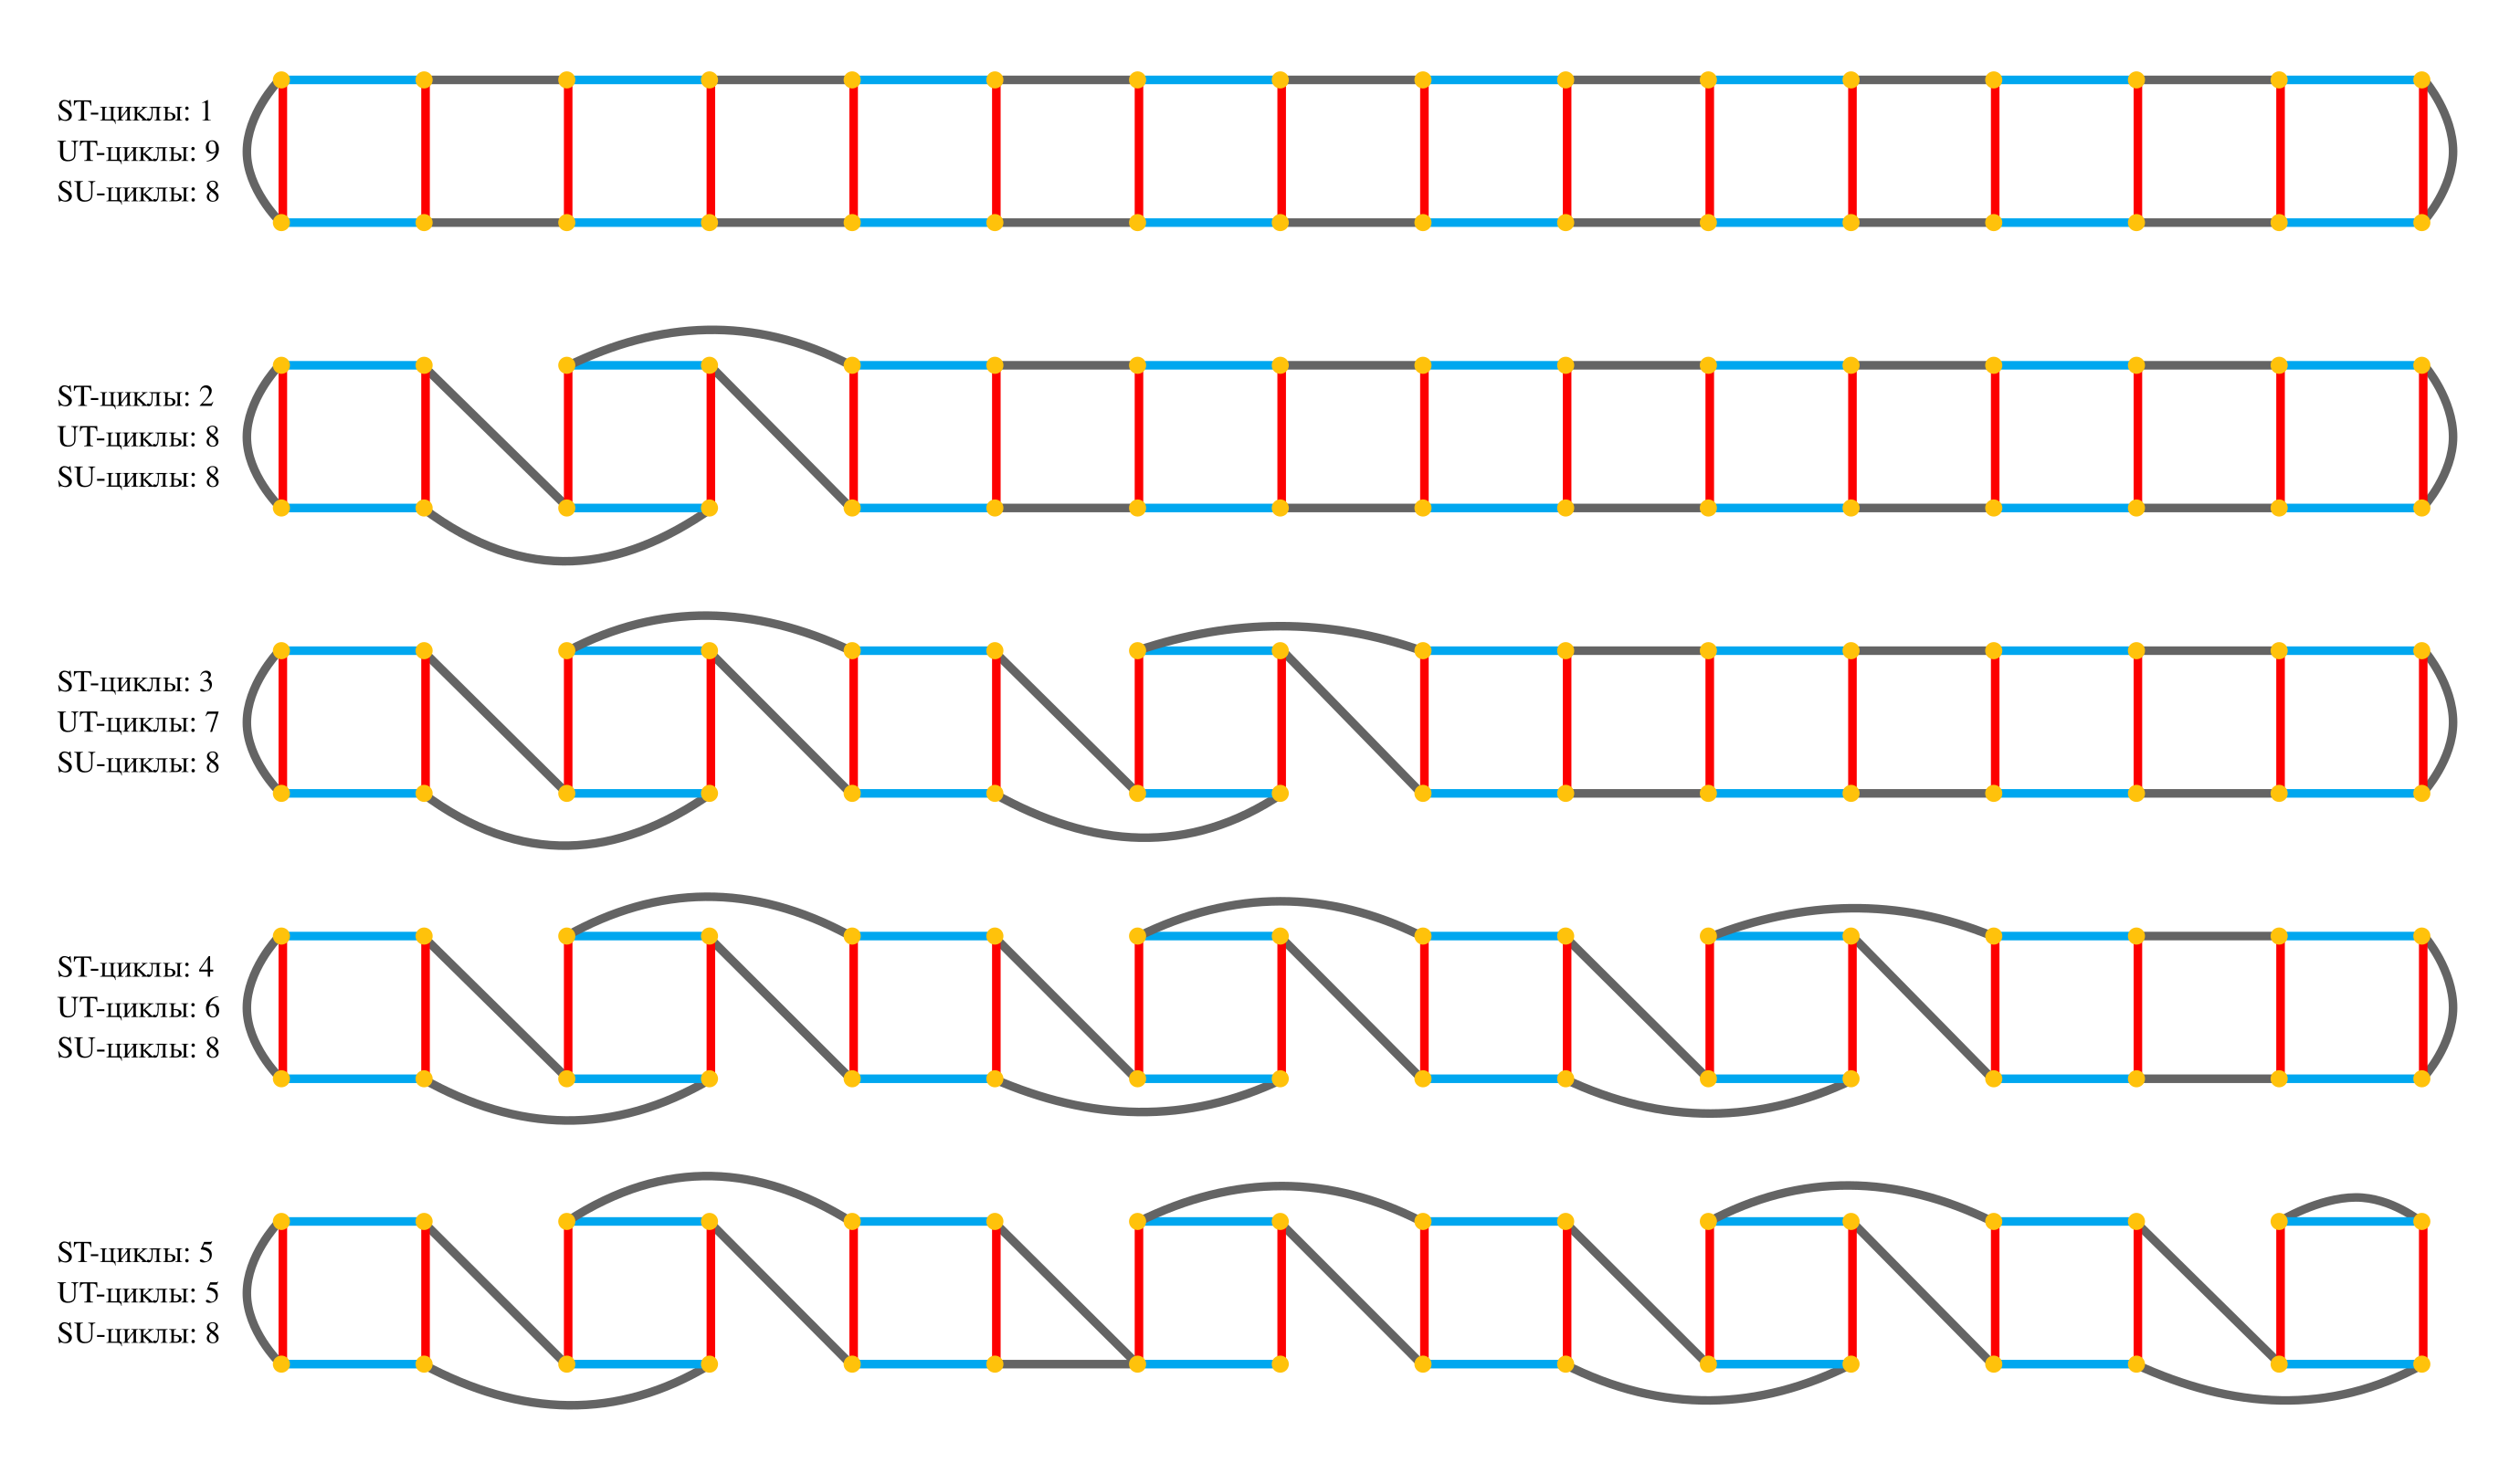
\includegraphics[width=\textwidth]{Spheres.png}
		\caption{Генератор графов для $e=2$ и $\sigma=8$ \label{overflow}}
	\end{figure}
	\subsection{Генератор графов по заданной характеристике Эйлера и числу сёдел}
	\hspace{0.5 cm} Для дальнейшей проверки алгоритма на корректность потребуется генерировать корректные трёхцветные графы со всевозможным количеством стоков и источников, такие, что соответствующие им градиентно-подобные каскады расположены на сфере, по заданному числу сёдел $\sigma$. Изложенную ниже генерацию можно обобщить для генерации трёхцветных графов, такие, что соответствующие им градиентно-подобные каскады расположены на ориентируемой поверхности, определяемой характеристикой Эйлера $e$.
	\par Из определения 10 известно, что длина SU-циклов корректного трёхцветного графа равна 4, причём количество SU-циклов равно числу сёдел $\sigma$. Тогда расположим <<квадраты>> SU-циклов, верхнее и нижнее ребро которых имеют одинаковый цвет для всех <<квадратов>> (будем считать, что верхние и нижние ребра - s-рёбра), в ряд и будем проводить из каждой вершины рёбра цвета t. Далее будем соединять t-ребром с ближайшей вершиной ближайшего соседнего <<квадрата>> SU-цикла, кроме первых 2 и последних 2 вершин, которые соединяются между собой соответственно. Получили тривиальный пример графа с числом SU-циклов, равному $\sigma$, числом ST-циклов, равному $1$, и числом UT-циклов, равному $\sigma+1$.
	\par Увеличим количество ST-циклов на 1 и уменьшим количество UT-циклов на 1. Это можно сделать из построенного выше тривиального графа при помощи переподвязок t-циклов. Переподвязывать t-циклы будем следующим способом: возьмём чётный по счёту <<квадрат>> и перекрасим s-рёбра в u-рёбра и наоборот. Одна такая переподвязка увеличивает количество ST-циклов на 1 и уменьшает количество UT-циклов на 1.
	\par Проводя такие переподвязки на чётных <<квадратах>> по одной поверх друг друга, сгенерируем циклы, для которых количество ST-циклов принимает значения (с учётом тривиального графа) $\{1,~...~, [\sigma/2]\}$, а количество UT-циклов $\{[(\sigma + 1)/2],~...~, \sigma+1\}$.
	\par Ниже приведены примеры построения трёхцветных графов при $\sigma=8$ и $e=0$ и $e=-2$ для рис. 3 и для рис. 4 соответственно.
	\begin{figure}[h!]
	\centering
	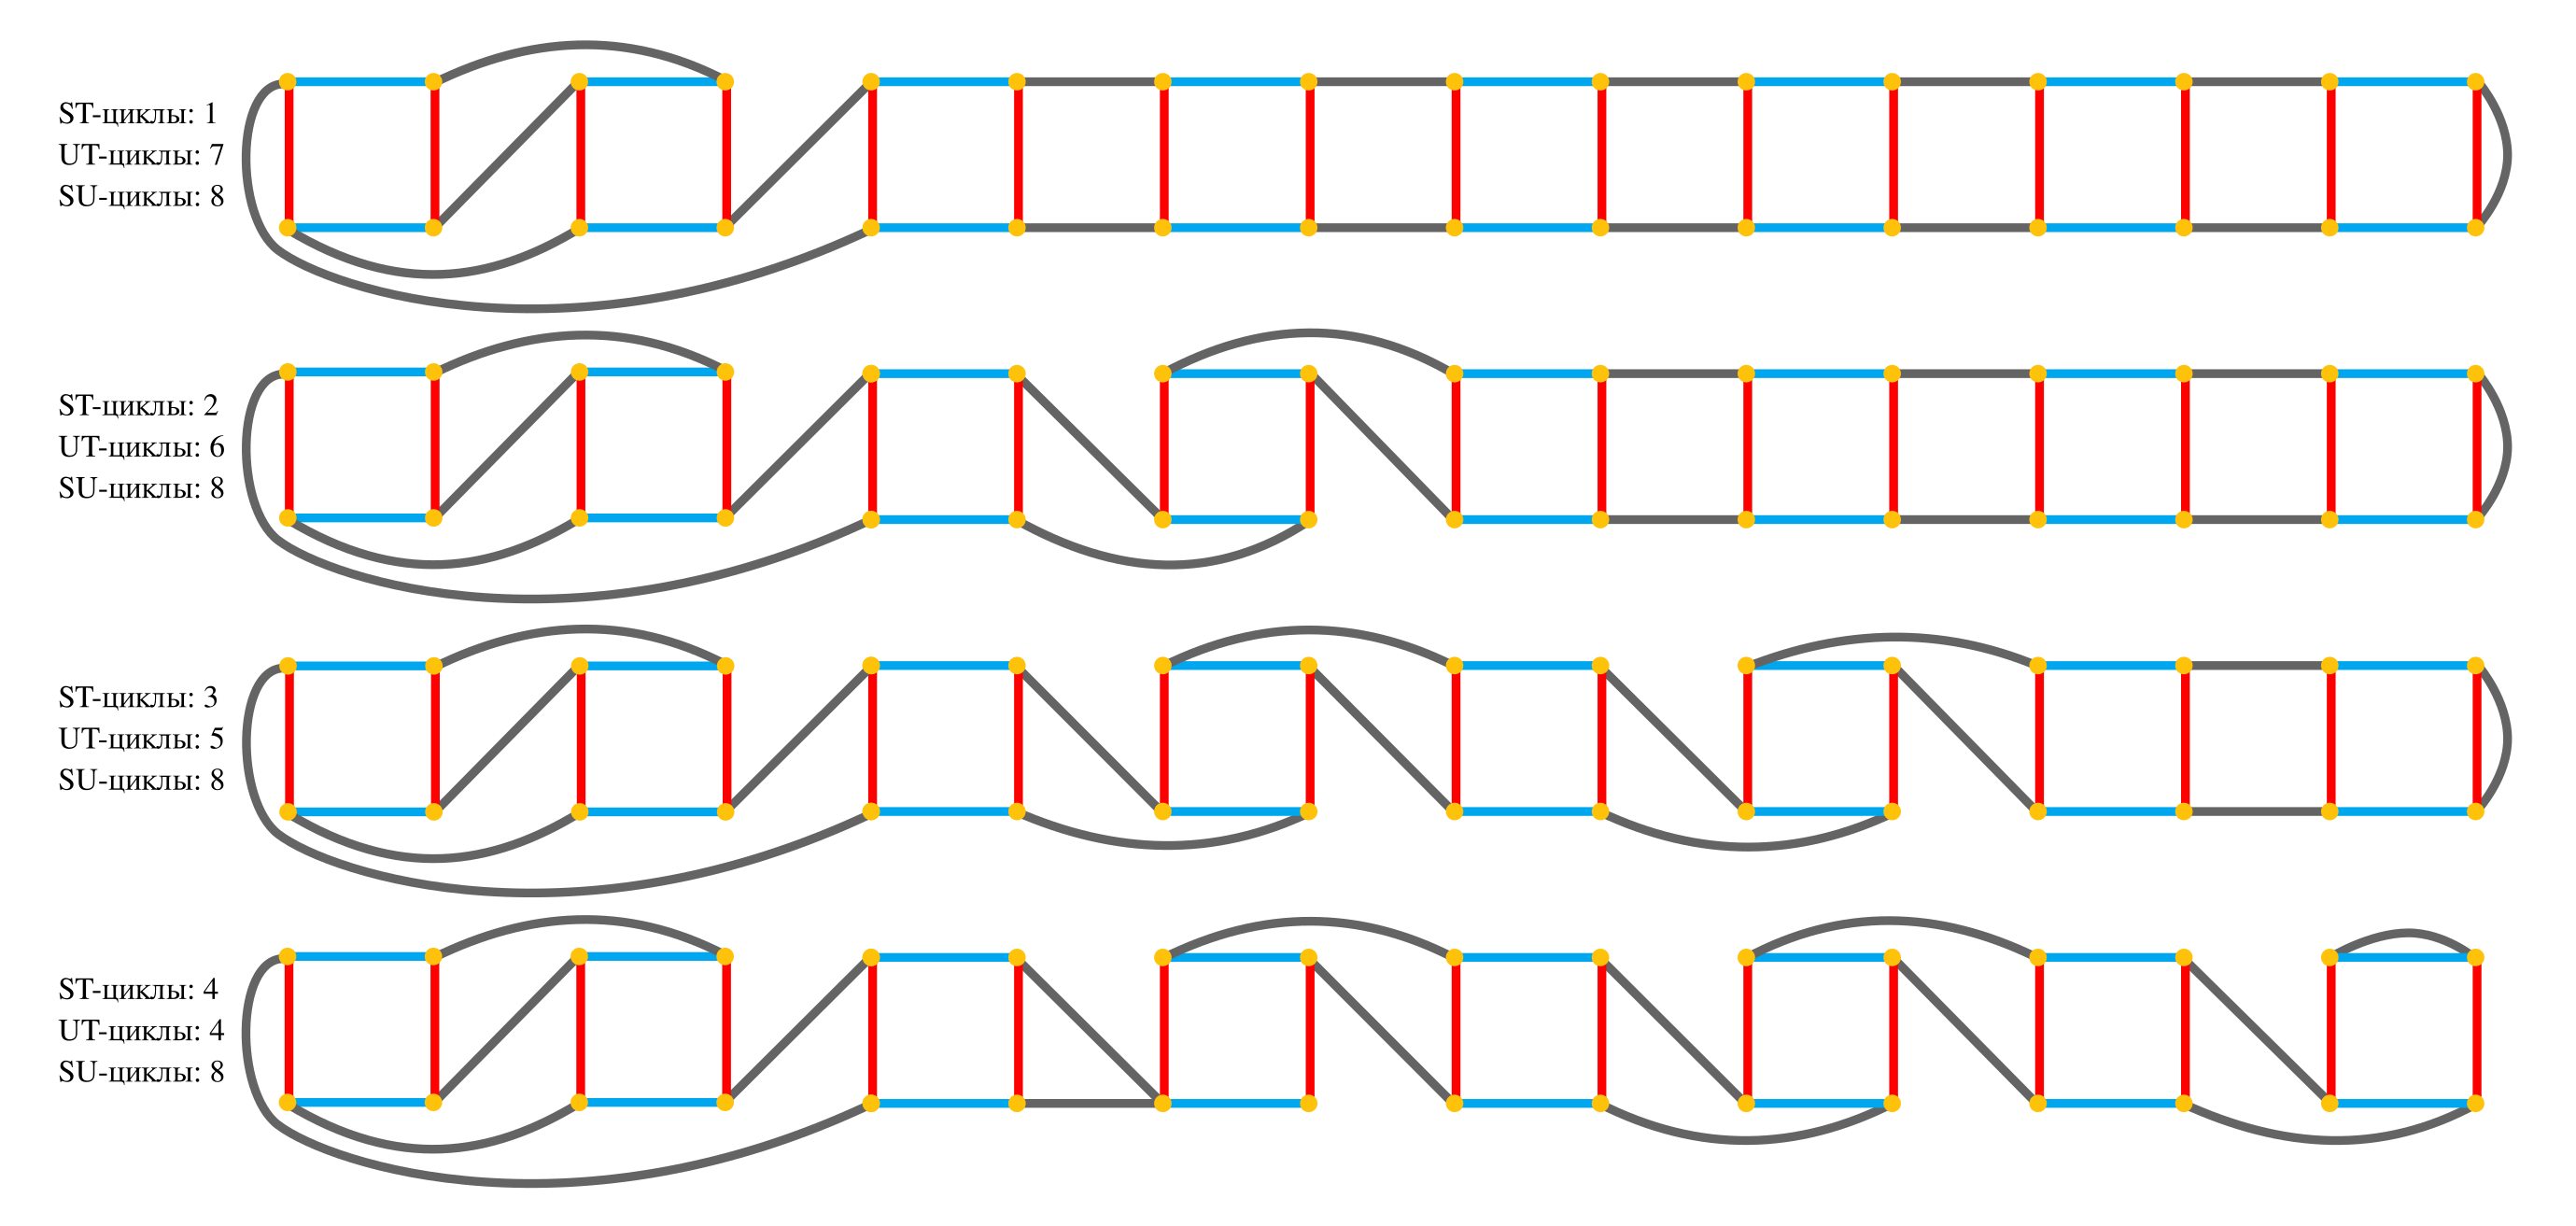
\includegraphics[width=\textwidth]{Torus.png}
	\caption{Генератор графов для $e=0$ и $\sigma=8$ \label{overflow}}
	\end{figure}
	\begin{figure}[h!]
	\centering
	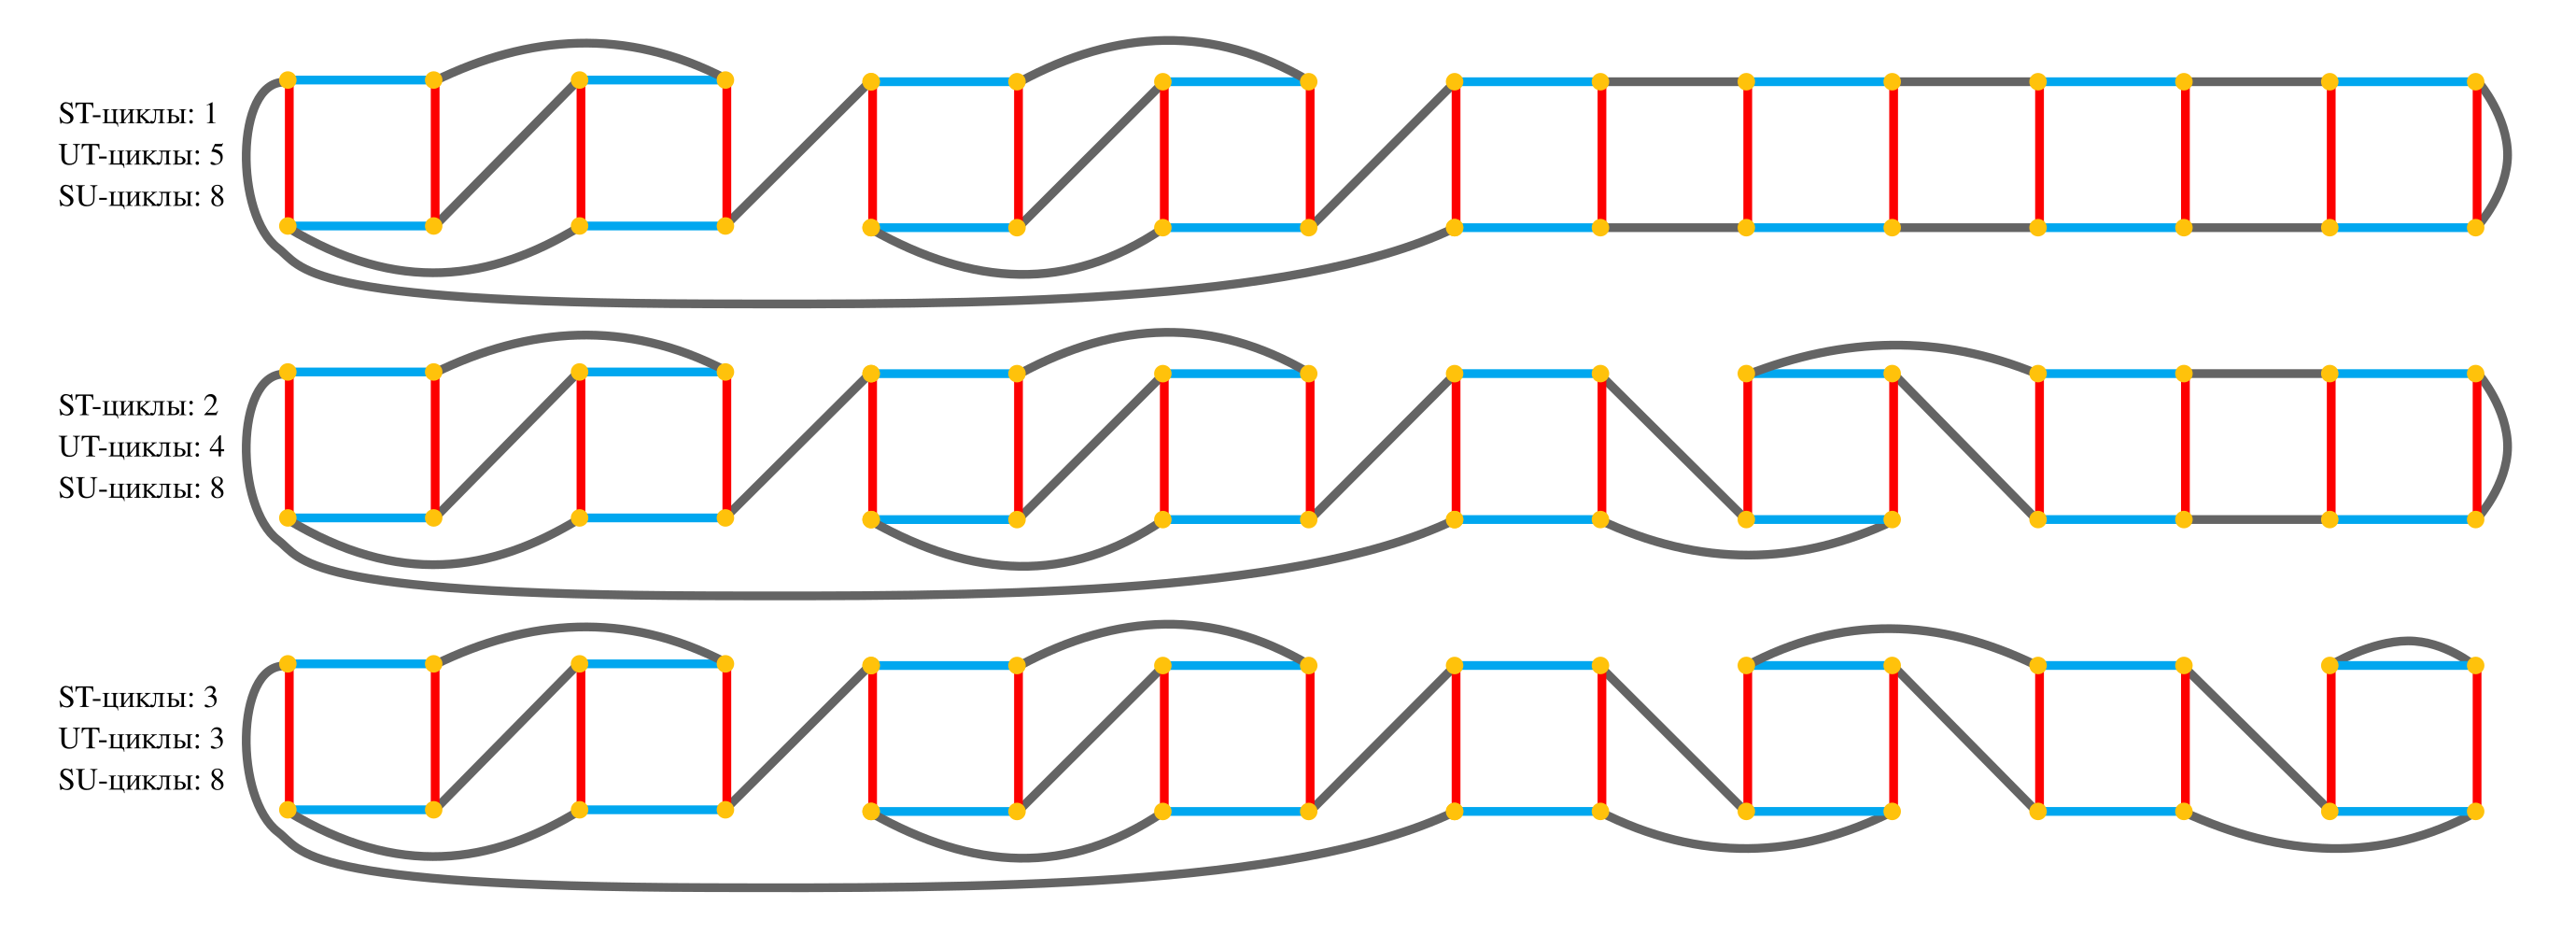
\includegraphics[width=\textwidth]{Double Torus.png}
	\caption{Генератор графов для $e=-2$ и $\sigma=8$ \label{overflow}}
	\end{figure}
	\subsection{Поиск соседних неподвижных точек}
	\hspace{0.5 cm} Нам дан корректный трёхцветный граф, для дальнейшей визуализации динамической системы для каждой неподвижной точки необходимо найти соседние, то есть соединённые с данной неподвижной точкой сепаратрисой, неподвижные точки. Для этого реализуем функцию $find \textunderscore neighbors$, которая принимает на вход корректный трёхцветный граф, а выдаёт вектор, состящий из стоков, сёдел и источников, а также их соседей в правильной последовательности.
	\par Для начала найдём все ST-, UT-, SU-циклы в исходном графе. Напомним, что каждый ST-цикл соответствует источнику, UT-цикл - стоку, SU-цикл - седлу. Из построения трёхцветного графа следует, что циклы имеют общее красное или синее ребро тогда и только тогда, когда неподвижные точки, представляющие эти циклы, соединены сепаратрисой, причём порядок обхода сепаратрис вокруг неподвижной точки соответствует порядку обхода рёбер графа, а также что одно ребро лежит ровно в двух двухцветных циклах, поэтому, найдя все двухцветные циклы, будем идти по ним в порядке обхода и для красных и синих рёбер будем смотреть, в каком ещё двухцветном цикле они лежат, далее сопоставляем новому двухцветному циклу для ребра неподвижную точку, соответствующую этому циклу. Проделаем это для всех неподвижных точек, получим искомый вектор.
	\subsection{Нахождение сепаратрис}
	\hspace{0.5 cm} Представим сферу как прямоугольник $[-90, 90]$ x $[0, 360]$, где все точки из отрезка $-90$ х $[0, 360]$ и из отрезка $90$ x $[0, 360]$ отождествлены между собой. Впоследствии при визуализации этот прямоугольник будем отображать на сферу по формуле:
	$$ \begin{cases}
		x = r * sin(\psi) * cos(\phi)\\
		x = r * sin(\psi) * sin(\phi)\\
		x = r * cos(\psi)
	\end{cases} $$ Сепаратрисы будем представлять как пары, состоящие из цвета сепаратрисы, красная или синяя, и вектора координат, содержащего $a, a0, b, b0$ и при этом заданной формулой:
	$$ \begin{cases}
		x = a * t + a_0\\
		y = b * t + b_0
	\end{cases} $$ где t $\in [0, 1]$.
	\begin{figure}[h]
		\centering
		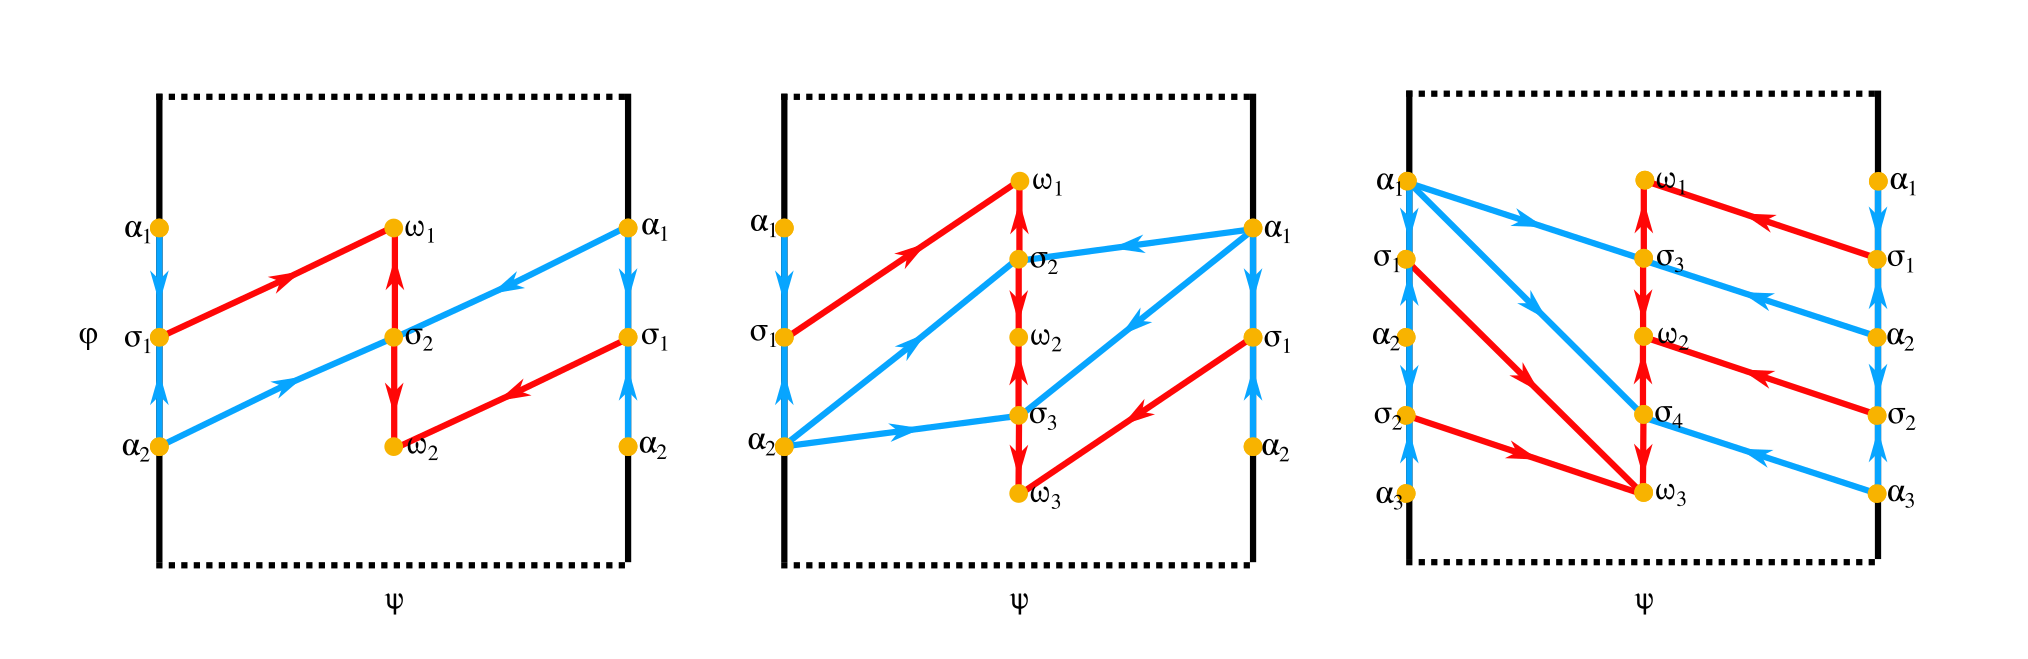
\includegraphics[width=\textwidth]{Projections.png}
		\caption{Представление каскада на сфере. \label{overflow}}
	\end{figure}
	\par Для нахождения координат сепаратрис на сфере реализована функция \\ $find \textunderscore separatres \textunderscore coords$, она принимает на вход изначальный граф. Функция сначала запускает описанную выше функцию $find \textunderscore neighbors$ и находит соседние неподвижные точки для каждой неподвижной точки. Напомним, что возвращаемый функцией $find \textunderscore neighbors$ вектор устроен так, что он для каждой неподвижной точки содержит информацию о том, чем является неподвижная точка: стоком, источником или седлом. Функция $find \textunderscore separatres \textunderscore coords$ проходит по вектору с соседями и выявляет набор источников и сёдел, которые должны быть расположены на краях прямоугольника, расположенных последовательно. Делает она это так: заходим в первый источник, ищем соседа-селдо, далее для этого седла ищем соседа-источник, которого у нас ещё нет в последовательности, далее для источника ищём соседа-седло, которого ещё не посетили, так повторяем до тех пор, пока не пройдём через все источники. После этого, функция аналогично выявляет расположенные последовательно оставшиеся стоки и сёдла, которые должны лежать в центре прямоугольника. Параллельно с этим функция для каждой неподвижной точки запоминает её координаты на этом прямоугольнике.
	\par После того, как координаты неподвижных точек найдены, функция начинает поиск координат сепаратрис. Для этого используется вспомогательная функция $find \textunderscore sep$. Она сначала находит координаты сепаратрис, расположенных по центру и с краю, там достаточно тривиальное расположение сепаратрис. После этого, функция пытается нарисовать сепаратрисы слева от центра: если отдельно взятая сепаратриса не пересеклась с остальными сепаратрисами, нарисованными справа, то рисуем её, если пересеклась, то переносим её в правую от центра часть. Для правой части отрисовываем все сепаратрисы, если какая-то пересеклась, то отражаем порядок и координаты неподвижных точек, распоженных по центру, и отрисовываем заново.
	\par Полученные координаты сепаратрис уже отдельно от файла, в файле $main.cpp$, передаём в текстовый документ, который затем будет прочтён из файла с визуализацией.
	\par Пересечение сепатарис находится при помощи функции $is \textunderscore separatres \textunderscore cross$, которая принимает на вход координаты двух сепаратрис, которые кеобходимо проверить на пересечение. Проверка сепаратрис на пересечение производится при помощи перебора всех возможных случаев (таких как пересечение, совпадение, параллельность) и переходом от параметрического задания прямой к каноническому, что при приравнивании поможет найти точку пересечения этих прямых. Если точка лежит на отрезке, то сепаратрисы пересеклись, если нет, то не пересеклись. При пересечении функция возвращает булевое значение True, в противном случае она возвращает False.
	\subsection{Unit-тестирование}
	\hspace{0.5 cm} Для стабильной работы программы при изменении в дальнейшем в каталоге под названием $graph \textunderscore algorithms \textunderscore unit \textunderscore test$ содержатся файлы, в которых написаны unit-тесты для различных функций. Если при изменении программа будет работать неправильно, то unit-тесты распознают аномалии.
	\newpage
	\section{Графическая часть}
	\subsection{Работа с библиотекой Manim}
	\hspace{0.5 cm} Графическая часть программы, написанная в файле draw.py, отвечает за генерацию 3D-изображения дискретной динамической системы на сфере.
	\par В файле определён класс DynamicalSystemSphere, который в дальнейшем будет указываться при запуске графической части.
	\par Графическая часть работает по следующему алгоритму:
	\par 1) Считывается информация о сепаратрисах, полученная в результате запуска алгоритмической части;
	\par 2) Объявляется функция $func \textunderscore sphere$, задающая параметрически поверхность сферы:
	$$ \begin{cases}
		x = r * cos(u) * sin(v) - x_0\\
		y = r * sin(u) * sin(v) - y_0\\
		z = r * cos(v) - z_0
	\end{cases} $$
	\par 3) Объявляется функция $construct$, которая отвечает непосредственно за генерацию 3D-изображения. При помощи библиотеки Manim создаются поверхность сферы и оси OX, OY и OZ. Далее каждая сепаратриса, разбитая на 3 равные части, отличающиеся по цвету: более яркий красный и синий цвет соответствуют близости к стокам и источникам соответственно, а бледные оттенки этих цветов соответствуют близости к седлу, по отдельности добавляется на поверхность сферы.
	\par Cепаратриса, заданная параметрически на прямоугольнике значениями $a, a0, b, b0$, отображается на поверхность сферы по правилу:
	$$ \begin{cases}
		x = cos(pi * (t * b + b_0) / 180) * sin(pi * (t * a + a_0) / 180)\\
		y = cos(pi * (t * b + b_0) / 180) * cos(pi * (t * a + a_0) / 180)\\
		z = sin(pi * (t * b + b_0) / 180)
	\end{cases} $$ где t принадлежит [0, 1] (причём для создания более <<говорящей>> картинки для различных оттенков сепаратрисы отрезок разбивается на 3 равные части, каждая из которых отображается независимо от остальных).
	\par Для получения объёмного и <<говорящего>> изображения объявляется полный оборот камеры вокруг сферы.
	\subsection{Запуск и результат работы программы}
	\hspace{0.5 cm} Для запуска генерации 3D-изображения необходимо:
	\par 1) При помощи терминала установить библиотеку Manim на компьютер, если эта библиотека ещё не установлена.
	\par 2) Предварительно запустить алгоритмическую часть с введённым в неё корректным трёхцветным графом.
	\par 3) При помощи терминала перейти в каталог с файлом draw.py.
	\par 4) Запустить графическую часть при помощи команды:
	\par manim -pqh draw.py DynamicalSystemSphere - для генерации изображения высокого качества;
	\par manim -pql draw.py DynamicalSystemSphere - для генерации изображения низкого качества.
	\section{Ссылка на репозиторий в Github}
	Ссылка на репозиторий: $https://github.com/dan1lka257/graphs \textunderscore and \textunderscore algorithms/tree/main$
	\section{Код графической части}
	\begin{lstlisting}[language=Python]
from manim import *

class DynamicalSystemSphere(ThreeDScene):
	separatress = []
	with open('../separatres.txt') as file:
	lines = [line.rstrip() for line in file]
	for line in lines:
	separatress.append([line[0]] + list(map(int, line[2:].split(' '))))
	
	def func_sphere(self, u, v, radius = 1):
		sphereCentre = np.array([0, 0, 0])
		return radius * np.array([np.cos(u) * np.sin(v) - sphereCentre[0]/radius,
		np.sin(u) * np.sin(v) - sphereCentre[1]/radius,
		np.cos(v) - sphereCentre[2]/radius])
	
	def construct(self):
		rng = 7
		axes = ThreeDAxes(
			x_range=[-rng, rng], y_range=[-rng, rng], z_range=[-rng, rng],
			x_length=rng, y_length=rng, z_length=rng
		)
		x_label = axes.get_x_axis_label(Tex("x"))
		y_label = axes.get_y_axis_label(Tex("y"))
		z_label = axes.get_z_axis_label(Tex("z"))
		mainSphere = Surface(
			lambda u, v: axes.c2p(*self.func_sphere(u, v, rng)),
			u_range=[0, TAU],
			v_range=[0, TAU],
			resolution=32, fill_opacity=0.1, checkerboard_colors=['#29ABCA', '#236B8E'], stroke_color=BLACK, stroke_width=0.1
		)
		for sep in self.separatress:
			u_sep1 = ParametricFunction(
			lambda t: (0.5 * rng) * np.array([
			np.cos(np.pi * (t * sep[3] + sep[4]) / 180) * np.sin(np.pi * (t * sep[1] + sep[2]) / 180),
			np.cos(np.pi * (t * sep[3] + sep[4]) / 180) * np.cos(np.pi * (t * sep[1] + sep[2]) / 180),
			np.sin(np.pi * (t * sep[3] + sep[4]) / 180)
			]), color=RED_A if sep[0]=='u' else BLUE_A, t_range = np.array([0, 1/3, 0.01])
			)
			u_sep1.set_z_index(mainSphere.z_index)
			self.add(u_sep1)
			
			u_sep2 = ParametricFunction(
			lambda t: (0.5 * rng) * np.array([
			np.cos(np.pi * (t * sep[3] + sep[4]) / 180) * np.sin(np.pi * (t * sep[1] + sep[2]) / 180),
			np.cos(np.pi * (t * sep[3] + sep[4]) / 180) * np.cos(np.pi * (t * sep[1] + sep[2]) / 180),
			np.sin(np.pi * (t * sep[3] + sep[4]) / 180)
			]), color=RED_C if sep[0]=='u' else BLUE_C, t_range = np.array([1/3, 2/3, 0.01])
			)
			u_sep2.set_z_index(mainSphere.z_index)
			self.add(u_sep2)
			
			u_sep3 = ParametricFunction(
			lambda t: (0.5 * rng) * np.array([
			np.cos(np.pi * (t * sep[3] + sep[4]) / 180) * np.sin(np.pi * (t * sep[1] + sep[2]) / 180),
			np.cos(np.pi * (t * sep[3] + sep[4]) / 180) * np.cos(np.pi * (t * sep[1] + sep[2]) / 180),
			np.sin(np.pi * (t * sep[3] + sep[4]) / 180)
			]), color=RED_E if sep[0]=='u' else BLUE_E, t_range = np.array([2/3, 1, 0.01])
			)
			u_sep3.set_z_index(mainSphere.z_index)
			self.add(u_sep3)
		# u_sep.rotate(PI / 4, about_point=[0, 0, 0], axis=RIGHT)
		self.add(axes, mainSphere, x_label, y_label, z_label)
		self.set_camera_orientation(theta=75*DEGREES, phi=75*DEGREES)
		self.begin_ambient_camera_rotation(rate=PI/10, about='theta')
		self.wait(10)
		self.stop_ambient_camera_rotation()
	\end{lstlisting}
	\section{Код алгоритмической части}
	\subsection{Поиск в ширину}
	\begin{lstlisting}[language=C++]
vector<int> bfs(int s, vector<vector<pair<int, char>>>& graph) {
	// BFS which find distance to other verticles
	int n = graph.size();
	vector<int> dist(n, INF);
	dist[s] = 0;
	queue<int> q;
	q.push(s);
	
	while (!q.empty()) {
		int v = q.front();
		q.pop();
		for (pair<int, char> u : graph[v]) {
			if (dist[u.first] > dist[v] + 1) {
				dist[u.first] = dist[v] + 1;
				q.push(u.first);
			}
		}
	}
	
	return dist;
}
	\end{lstlisting}
\subsection{Проверка на трёхцветность, неориентируемость и отсутствие петель}
\begin{lstlisting}[language=C++]
bool is_3_colored_and_non_oriented(vector<vector<pair<int, char>>>& graph) {
	// checks graph on tricolor and orientedness
	// 1 edge of each of 3 colors in one verticle
	for (int i = 0; i < graph.size(); i++) {
		// tricolor check
		int color_u = 0, color_s = 0, color_t = 0;
		for (int j = 0; j < graph[i].size(); j++) {
			if (graph[i][j].second == 'u') color_u += 1;
			if (graph[i][j].second == 's') color_s += 1;
			if (graph[i][j].second == 't') color_t += 1;
		}
		// orientedness check
		int oriented = 1;
		for (int j = 0; j < graph[i].size(); j++) {
			if (i != graph[graph[i][j].first][j].first) {
				oriented = 0;
			}
		}
		// no cycles with len = 1
		int has_no_cycles_with_len_1 = 1;
		for (int j = 0; j < graph[i].size(); j++) {
			if (i != graph[i][j].first) {
				has_no_cycles_with_len_1 = 0;
			}
		}
		if (!(color_u == 1 && color_s == 1 && color_t == 1)) {
			// Graph is not 3 colored
			return false;
		}
		if (!(oriented)) {
			// Graph is not oriented
			return false;
		}
		
		if (!(has_no_cycles_with_len_1)) {
			// Graph has cycles with len = 1
			return false;
		}
	}
	return true;
}
\end{lstlisting}
\subsection{Проверка на связность}
\begin{lstlisting}[language=C++]
bool is_connected(vector<vector<pair<int, char>>>& graph) {
	// checks graph is connected or not
	vector<int> dist = bfs(0, graph);
	int max_dist = 0;
	for (int j = 0; j < dist.size(); j++) {
		max_dist = max(max_dist, dist[j]);
	}
	if (max_dist == INF) {
		return false;
	}
	return true;
}
\end{lstlisting}
\subsection{Поиск цикла}
\begin{lstlisting}[language=C++]
vector<int> find_cycle(char color1, char color2, char prev_color, int cur_v, int prev_v, vector<vector<pair<int, char>>>& graph, vector<string>& color, vector<int>& parent) {
	// Standard cycle finding taking into account cycle's bicolor
	color[cur_v] = "grey";
	for (int i = 0; i < graph[cur_v].size(); i++) {
		if (graph[cur_v][i].second != prev_color && (graph[cur_v][i].second == color1 || graph[cur_v][i].second == color2)) {
			if (color[graph[cur_v][i].first] == "white") {
				parent.push_back(cur_v);
				return find_cycle(color1, color2, graph[cur_v][i].second, graph[cur_v][i].first, cur_v, graph, color, parent);
			}
			if (color[graph[cur_v][i].first] == "grey" && graph[cur_v][i].first != prev_v && cur_v != prev_v) {
				parent.push_back(cur_v);
				return parent;
			}
		}
	}
	parent.push_back(cur_v);
	color[cur_v] = "black";
	return parent;
}
\end{lstlisting}
\subsection{Поиск циклов}
\begin{lstlisting}[language=C++]
vector<vector<int>> find_cycles(vector<vector<pair<int, char>>>& graph, char color1, char color2) {
	// Find bicolored cycles in graph
	int n = graph.size();
	vector<int> used_v(n, 0);
	vector<vector<int>> cycles;
	for (int i = 0; i < n; i++) {
		if (!used_v[i]) {
			vector<string> color(n, "white");
			vector<int> parent;
			vector<int> cycle = find_cycle(color1, color2, 'o', i, i, graph, color, parent);
			if (cycle.empty()) {
				continue;
			}
			for (int j = 0; j < cycle.size(); j++) {
				used_v[cycle[j]] = 1;
			}
			cycles.push_back(cycle);
		}
	}
	return cycles;
}
\end{lstlisting}
\subsection{Проверка на допустимость}
\begin{lstlisting}[language=C++]
bool is_acceptable(vector<vector<pair<int, char>>>& graph) {
	// Lenght of su-cycle is equal 4, graph is connected, non_oriented and tricolored
	vector<vector<int>> cycles = find_cycles(graph, 's', 'u');
	bool su_cycle_is_4 = 1;
	for (int i = 0; i < cycles.size(); i++) {
		if (cycles[i].size() != 4) {
			su_cycle_is_4 = 0;
		}
	}
	return su_cycle_is_4 && is_connected(graph) && is_3_colored_and_non_oriented(graph);
}
\end{lstlisting}
\subsection{Подсчёт Эйлеровой характеристики}
\begin{lstlisting}[language=C++]
int count_euler_number(vector<vector<pair<int, char>>>& graph) {
	// Euler number = tu - su + st
	return find_cycles(graph, 'u', 't').size() - find_cycles(graph, 's', 'u').size() + find_cycles(graph, 's', 't').size();
}
\end{lstlisting}
\subsection{Проверка поверхности на ориентируемость}
\begin{lstlisting}[language=C++]
bool is_oriented_surface(vector<vector<pair<int, char>>>& graph) {
	// Graph is on oriented surface <=> length of all cycles is even
	// All cycles is even <=> any cycle from base of cycles is even
	vector<vector<int>> spanning_tree(graph.size(), vector<int> ());
	vector<int> visited(graph.size(), 0);
	// Creating spanning tree for future cycle finding
	for (int i = 0; i < graph.size(); i++) {
		vector<int> i_neighbors;
		for (int j = 0; j < graph[i].size(); j++) {
			if (visited[graph[i][j].first] == 0) {
				spanning_tree[i].push_back(graph[i][j].first);
				spanning_tree[graph[i][j].first].push_back(i);
				i_neighbors.push_back(j);
				visited[graph[i][j].first] = 1;
				visited[i] = 1;
			}
		}
	}
	vector<int> way_from_root = bfs(0, spanning_tree);
	// Finding base of cycles & checking if cycles is even
	vector<vector<int>> base;
	bool is_even_base = true;
	for (int i = 0; i < graph.size(); i++) {
		for (int j = 0; j < graph[i].size(); j++) {
			bool is_in = false;
			for (int k = 0; k < spanning_tree[i].size(); k++) {
				if (graph[i][j].first == spanning_tree[i][k]) {
					is_in = true;
					break;
				}
			}
			if (!is_in && (way_from_root[i] + way_from_root[graph[i][j].first] + 1) % 2 == 1) {
				is_even_base = false;
				cout << "!!!" << i << ":" << way_from_root[i] << " " << graph[i][j].first << ":" << way_from_root[graph[i][j].first] << "!!!";
				break;
			}
		}
		if (!is_even_base) {
			break;
		}
	}
	return is_even_base;
}
\end{lstlisting}
\subsection{Генератор трёхцветных графов}
\begin{lstlisting}[language=C++]
vector<vector<vector<pair<int, char>>>> graph_generator(int euler_number, int saddles) {
	vector<vector<vector<pair<int, char>>>> graphs(0);
	// Generating primal graph
	vector<vector<pair<int, char>>> graph(0);
	for (int i = 0; i < saddles * 4; i++) {
		vector<pair<int, char>> neighbours;
		if (i == 0) { // first verticle
			neighbours = { {i + 1, 't'}, {i + 2, 's'}, {i + 1, 'u'} };
		} else if (i == 1) { // second verticle
			neighbours = { {i - 1, 't'}, {i + 2, 's'}, {i - 1, 'u'} };
		} else if (i == saddles * 4 - 1) { // last verticle
			neighbours = { {i - 1, 't'}, {i - 2, 's'}, {i - 1, 'u'} };
		} else if (i == saddles * 4 - 2) { // penultimate verticle
			neighbours = { {i + 1, 't'}, {i - 2, 's'}, {i + 1, 'u'} };
		} else if (i % 4 == 0) {
			neighbours = { {i - 2, 't'}, {i + 2, 's'}, {i + 1, 'u'} };
		} else if (i % 4 == 1) {
			neighbours = { {i - 2, 't'}, {i + 2, 's'}, {i - 1, 'u'} };
		} else if (i % 4 == 2) {
			neighbours = { {i + 2, 't'}, {i - 2, 's'}, {i + 1, 'u'} };
		} else if (i % 4 == 3) {
			neighbours = { {i + 2, 't'}, {i - 2, 's'}, {i - 1, 'u'} };
		}
		graph.push_back(neighbours);
	}
	// operating with euler number
	if (2 - euler_number > saddles) {
		cout << "Uncorrect input: number of saddles must be lower or equal than (2 - euler_number)\n";
		return graphs;
	}
	for (int i = euler_number; i < 2; i += 2) {
		int j = 8 * (i - euler_number) / 2;
		if (euler_number == 0 && saddles == 2) { // usual torus
			graph[j][0].first = j + 1;
			graph[j + 1][0].first = (j + 1) - 1;
			graph[j + 2][0].first = (j + 2) + 4;
			graph[j + 3][0].first = (j + 3) + 1;
			graph[j + 4][0].first = (j + 4) - 1;
			graph[j + 5][0].first = (j + 5) + 2;
			graph[j + 6][0].first = (j + 6) - 4;
			graph[j + 7][0].first = (j + 7) - 2;
		} else if (i == euler_number) { // First step
			if (2 - euler_number < saddles) {
				graph[j][0].first = 8 * (2 - euler_number) / 2 + 1;
				graph[8 * (2 - euler_number) / 2 + 1][0].first = j;
			} else {
				graph[j][0].first = 8 * (2 - euler_number) / 2 - 1;
				graph[8 * (2 - euler_number) / 2 - 1][0].first = j;
			}
			graph[j + 1][0].first = (j + 1) + 4;
			graph[j + 2][0].first = (j + 2) + 4;
			graph[j + 3][0].first = (j + 3) + 1;
			graph[j + 4][0].first = (j + 4) - 1;
			graph[j + 5][0].first = (j + 5) - 4;
			graph[j + 6][0].first = (j + 6) - 4;
			graph[j + 7][0].first = (j + 7) + 1; // non-oriented graph
			graph[(j + 7) + 1][0].first = j + 7; // non-oriented graph
		} else if (i == 2 - 2 && 2 - euler_number == saddles) { // Last step
			graph[j][0].first = j - 1;
			graph[j + 1][0].first = (j + 1) + 4;
			graph[j + 2][0].first = (j + 2) + 4;
			graph[j + 3][0].first = (j + 3) + 1;
			graph[j + 4][0].first = (j + 4) - 1;
			graph[j + 5][0].first = (j + 5) - 4;
			graph[j + 6][0].first = (j + 6) - 4;
			graph[j + 7][0].first = 0;
		} else {
			graph[j][0].first = j - 1;
			graph[j + 1][0].first = (j + 1) + 4;
			graph[j + 2][0].first = (j + 2) + 4;
			graph[j + 3][0].first = (j + 3) + 1;
			graph[j + 4][0].first = (j + 4) - 1;
			graph[j + 5][0].first = (j + 5) - 4;
			graph[j + 6][0].first = (j + 6) - 4;
			graph[j + 7][0].first = (j + 7) + 1; // non-oriented graph
			graph[(j + 7) + 1][0].first = j + 7; // non-oriented graph
		}
	}
	graphs.push_back(graph);
	for (int i = (2 - euler_number) + 1; i < saddles; i += 2) {
		int j = i * 4;
		if (i == saddles - 1) {
			graph[j][0].first = j - 1;
			graph[j - 1][0].first = j;
			
			graph[j + 1][0].first = (j + 1) + 2; //equal
			graph[(j + 1) + 2][0].first = j + 1;
			
			
			graph[j + 2][0].first = (j + 2) - 4;
			graph[(j + 2) - 4][0].first = j + 2;
			
			graph[j + 3][0].first = (j + 3) - 2; // equal
			graph[(j + 3) - 2][0].first = j + 3;
		} else {
			graph[j][0].first = j - 1;
			graph[j - 1][0].first = j;
			
			graph[j + 1][0].first = (j + 1) + 4;
			graph[(j + 1) + 4][0].first = j + 1;
			
			
			graph[j + 2][0].first = (j + 2) - 4;
			graph[(j + 2) - 4][0].first = j + 2;
			
			graph[j + 3][0].first = (j + 3) + 1;
			graph[(j + 3) + 1][0].first = j + 3;
		}
		graphs.push_back(graph);
	}
	int fixed_size = graphs.size();
	for (int i = 0; i < fixed_size; i++) {
		vector<vector<pair<int, char>>> graph_reverse(0);
		graph_reverse.assign(graphs[i].begin(), graphs[i].end());
		for (int j = 0; j < graph_reverse.size(); j++) {
			int c = graph_reverse[j][1].first;
			graph_reverse[j][1].first = graph_reverse[j][2].first;
			graph_reverse[j][2].first = c;
		}
		graphs.push_back(graph_reverse);
	}
	return graphs;
}
\end{lstlisting}
\subsection{Поиск соседей}
\begin{lstlisting}[language=C++]
vector<pair<char, vector<int>>> find_neighbors(vector<vector<pair<int, char>>>& graph) {
	vector<pair<char, vector<int>>> cycles(0);
	// Sourses
	vector<vector<int>> cycles_st = find_cycles(graph, 's', 't');
	vector<pair<char, vector<int>>> a_cycles(0);
	for (int i = 0; i < cycles_st.size(); i++) {
		a_cycles.push_back(make_pair('a', cycles_st[i]));
	}
	// Drains
	vector<vector<int>> cycles_ut = find_cycles(graph, 'u', 't');
	vector<pair<char, vector<int>>> o_cycles(0);
	for (int i = 0; i < cycles_ut.size(); i++) {
		a_cycles.push_back(make_pair('o', cycles_ut[i]));
	}
	// Saddles
	vector<vector<int>> cycles_su = find_cycles(graph, 's', 'u');
	vector<pair<char, vector<int>>> s_cycles(0);
	for (int i = 0; i < cycles_su.size(); i++) {
		a_cycles.push_back(make_pair('s', cycles_su[i]));
	}
	// Uniting
	cycles.insert(cycles.end(), a_cycles.begin(), a_cycles.end());
	cycles.insert(cycles.end(), o_cycles.begin(), o_cycles.end());
	cycles.insert(cycles.end(), s_cycles.begin(), s_cycles.end());
	// Cycles-neighbors finding
	int alphas = cycles_st.size();
	int omegas = cycles_ut.size();
	int sigmas = cycles_su.size();
	vector<pair<char, vector<int>>> neighbors(0);
	for (int i = 0; i < cycles.size(); i++) { // O(n^2)
		vector<int> empty_vector(0);
		neighbors.push_back(make_pair(cycles[i].first, empty_vector));
		char i_cycle_type = cycles[i].first;
		for (int j = 0; j < cycles[i].second.size(); j++) {
			int a1 = cycles[i].second[j];
			int a2 = cycles[i].second[(j + 1) % cycles[i].second.size()];
			bool is_found = false;
			for (int k = 0; k < cycles.size(); k++) {
				char k_cycle_type = cycles[k].first;
				if (((i_cycle_type == 'a' && k_cycle_type == 's' && graph[a1][1].first == a2)) || (i_cycle_type == 'o' && k_cycle_type == 's' && graph[a1][2].first == a2) || (i_cycle_type == 's' && ((k_cycle_type == 'a' && graph[a1][1].first == a2) || (k_cycle_type == 'o' && graph[a1][2].first == a2)))) {
					if (k == i) {
						continue;
					}
					for (int t = 0; t < cycles[k].second.size(); t++) {
						int b1 = cycles[k].second[t];
						int b2 = cycles[k].second[(t + 1) % cycles[k].second.size()];
						if ((a1 == b1 && a2 == b2) || (a1 == b2 && a2 == b1)) {
							neighbors[i].second.push_back(k);
							is_found == true;
							break;
						}
					}
					if (is_found) {
						break;
					}
				}
			}
			if (cycles[i].second.size() == 2) {
				break;
			}
		}
	}
	return neighbors;
}
\end{lstlisting}
\subsection{Проверка сепаратрис на пересечение}
\begin{lstlisting}[language=C++]
bool is_separatres_cross(vector<float> sep1, vector<float> sep2) {
	float a = sep1[0], a0 = sep1[1], b = sep1[2], b0 = sep1[3], t1 = sep1[4], t2 = sep1[5];
	float c = sep2[0], c0 = sep2[1], d = sep2[2], d0 = sep2[3], k1 = sep2[4], k2 = sep2[5];
	float max_t = max(t1, t2);
	float min_t = min(t1, t2);
	t1 = min_t;
	t2 = max_t;
	float max_k = max(k1, k2);
	float min_k = min(k1, k2);
	k1 = min_k;
	k2 = max_k;
	if ((a0 != c0 || b0 != d0) && a*d == b*c) {
		return false; // parallel
	}
	if (a0 == c0 && b0 == d0 && a*d == b*c && t2 > k1 && k2 > t1) {
		return true; // coincide
	} else if (a0 == c0 && b0 == d0 && a*d == b*c) {
		return false; // lying on one line
	}
	float y_cross = (b * d * c0 - b * c * d0 - b * d * a0 + d * a * b0) / (d * a - b * c); // calculated before (linear algebra)
	float x_cross;
	float t_cross, k_cross;
	if (b != 0) {
		t_cross = (y_cross - b0) / b; // calculated before (linear algebra)
	} else {
		x_cross = (c * y_cross - c * d0) / d + c0; // calculated before (linear algebra)
		t_cross = (x_cross - a0) / a; // calculated before (linear algebra)
	}
	if (d != 0) {
		k_cross = (y_cross - d0) / d; // calculated before (linear algebra)
	} else {
		x_cross = (a * y_cross - a * b0) / b + a0; // calculated before (linear algebra)
	}
	bool is_crossing = (t1 < t_cross && t_cross < t2) && (k1 < k_cross && k_cross < k2);
	return is_crossing;
}
\end{lstlisting}
\subsection{Поиск сепаратрис 1}
\begin{lstlisting}[language=C++]
vector<pair<char, vector<float>>> find_sep(int side_len, int center_len, vector<pair<char, int>> sourse_order, vector<pair<char, int>> drain_order, vector<pair<char, vector<int>>> neighbors) {
	vector<pair<int, pair<float, float>>> side(side_len);
	vector<pair<int, pair<float, float>>> center(center_len);
	for (int i = 1; i < side_len + 1; i++) {
		float y = -180 * i / (side_len + 1) + 90;
		side[i - 1] = (make_pair(sourse_order[i - 1].second, make_pair(0, y)));
	}
	for (int i = 1; i < center_len + 1; i++) {
		float y = -180 * i / (center_len + 1) + 90;
		center[i - 1] = (make_pair(drain_order[i - 1].second, make_pair(180, y)));
	}
	
	vector<pair<char, vector<float>>> left;
	vector<pair<char, vector<float>>> right;
	for (int i = 0; i < side.size(); i++) {
		if (i % 2) {
			vector<float> coords = {side[i - 1].second.first - side[i].second.first, side[i].second.first, side[i - 1].second.second - side[i].second.second, side[i].second.second, 0, 1};
			right.push_back(make_pair('s', coords));
			coords = {side[i + 1].second.first - side[i].second.first, side[i].second.first, side[i + 1].second.second - side[i].second.second, side[i].second.second, 0, 1};
			right.push_back(make_pair('s', coords));
		}
	}
	for (int i = 0; i < center.size(); i++) {
		if (i % 2) {
			vector<float> coords = {center[i - 1].second.first - center[i].second.first, center[i].second.first, center[i - 1].second.second - center[i].second.second, center[i].second.second, 0, 1};
			right.push_back(make_pair('u', coords));
			coords = {center[i + 1].second.first - center[i].second.first, center[i].second.first, center[i + 1].second.second - center[i].second.second, center[i].second.second, 0, 1};
			right.push_back(make_pair('u', coords));
		}
	}
	
	for (int i = 0; i < sourse_order.size(); i++) {
		if (true /*sourse_order[i].first == 's'*/) {
			for (int j = 0; j < neighbors[sourse_order[i].second].second.size(); j++) {
				if (neighbors[sourse_order[i].second].second[j] == sourse_order[(i - 1 + sourse_order.size()) % sourse_order.size()].second || neighbors[sourse_order[i].second].second[j] == sourse_order[(i + 1 + sourse_order.size()) % sourse_order.size()].second) {
					continue;
				}
				float xi, yi, xj, yj;
				for (int k = 0; k < side.size(); k++) {
					if (side[k].first == sourse_order[i].second) {
						xi = side[k].second.first;
						yi = side[k].second.second;
						break;
					}
				}
				for (int k = 0; k < center.size(); k++) {
					if (center[k].first == neighbors[sourse_order[i].second].second[j]) {
						xj = center[k].second.first;
						yj = center[k].second.second;
						break;
					}
				}
				vector<float> sep = {xj - xi, xi, yj - yi, yi, 0, 1};
				bool is_crossing = false;
				for (int k = 0; k < left.size(); k++) {
					if (is_separatres_cross(sep, left[k].second)) {
						is_crossing = true;
						break;
					}
				}
				if (is_crossing) {
					sep = {xj - (xi + 360), (xi + 360), yj - yi, yi, 0, 1};
					if (sourse_order[i].first == 's') {
						right.push_back(make_pair('u', sep));
					} else if (sourse_order[i].first == 'a') {
						sep = {xi - xj, xj, yi - yj, yj, 0, 1};
						right.push_back(make_pair('s', sep));
					}
				} else {
					if (sourse_order[i].first == 's') {
						left.push_back(make_pair('u', sep));
					} else if (sourse_order[i].first == 'a') {
						sep = {xi - xj, xj, yi - yj, yj, 0, 1};
						left.push_back(make_pair('s', sep));
					}
				}
			}
		}
	}
	
	for (int i = 0; i < drain_order.size(); i++) {
		if (drain_order[i].first == 's') {
			for (int j = 0; j < neighbors[drain_order[i].second].second.size(); j++) {
				if (neighbors[drain_order[i].second].second[j] == drain_order[(i - 1 + drain_order.size()) % drain_order.size()].second || neighbors[drain_order[i].second].second[j] == drain_order[(i + 1 + drain_order.size()) % drain_order.size()].second) {
					continue;
				}
				float xi, yi, xj, yj;
				for (int k = 0; k < center.size(); k++) {
					if (center[k].first == drain_order[i].second) {
						xi = center[k].second.first;
						yi = center[k].second.second;
						break;
					}
				}
				for (int k = 0; k < side.size(); k++) {
					if (side[k].first == neighbors[drain_order[i].second].second[j]) {
						xj = side[k].second.first;
						yj = side[k].second.second;
						break;
					}
				}
				vector<float> sep = {xj - xi, xi, yj - yi, yi, 0, 1};
				bool is_crossing = false;
				for (int k = 0; k < left.size(); k++) {
					if (is_separatres_cross(sep, left[k].second)) {
						is_crossing = true;
					}
				}
				if (is_crossing) {
					sep = {(xj + 360) - xi, xi, yj - yi, yi, 0, 1};
					right.push_back(make_pair('s', sep));
				} else {
					left.push_back(make_pair('s', sep));
				}
			}
		}
	}
	left.insert(left.end(), right.begin(), right.end());
	return left;
}
\end{lstlisting}
\subsection{Поиск сепаратрис 2}
\begin{lstlisting}[language=C++]
vector<pair<char, vector<float>>> find_separatres_coords(vector<vector<pair<int, char>>>& graph) {
	vector<pair<char, vector<int>>> neighbors;
	neighbors = find_neighbors(graph);
	vector<pair<int, vector<int>>> sourses;
	vector<pair<int, vector<int>>> saddles;
	vector<pair<int, vector<int>>> drains;
	// Count sourses, saddles and drains number
	for (int i = 0; i < neighbors.size(); i++) {
		if (neighbors[i].first == 'a') {
			sourses.push_back(make_pair(i, neighbors[i].second));
		} else if (neighbors[i].first == 's') {
			saddles.push_back(make_pair(i, neighbors[i].second));
		} else if (neighbors[i].first == 'o') {
			drains.push_back(make_pair(i, neighbors[i].second));
		}
	}
	int sourses_num = sourses.size();
	int saddles_num = saddles.size();
	int drains_num = drains.size();
	int side_len = 2 * sourses_num - 1;
	int center_len = 2 * drains_num - 1;
	vector<pair<char, int>> sourse_order;
	pair<int, vector<int>> curr_v = sourses[0];
	sourse_order.push_back(make_pair('a', curr_v.first));
	while (sourse_order.size() != side_len) {
		for (int i = 0; i < curr_v.second.size(); i++) {
			bool is_saddle = false;
			int saddle_index = -1;
			int saddle_value = -1;
			for (int j = 0; j < saddles.size(); j++) {
				if (saddles[j].first == curr_v.second[i]) {
					is_saddle = true;
					saddle_value = saddles[j].first;
					saddle_index = j;
					break;
				}
			}
			if (is_saddle) {
				bool already_was = false;
				for (int j = 0; j < sourse_order.size(); j++) {
					if (saddle_value == sourse_order[j].second) {
						already_was = true;
					}
				}
				if (already_was) {
					continue;
				}
				int sourse_index1 = -1;
				int sourse_value1 = -1;
				int sourse_index2 = -1;
				int sourse_value2 = -1;
				for (int t = 0; t < saddles[saddle_index].second.size(); t++) {
					// there could be break_factor to speed up cycle
					for (int j = 0; j < sourses.size(); j++) {
						if (sourses[j].first == saddles[saddle_index].second[t]) {
							if (sourse_index1 == -1) {
								sourse_value1 = sourses[j].first;
								sourse_index1 = j;
							} else if (sourse_index2 == -1) {
								sourse_value2 = sourses[j].first;
								sourse_index2 = j;
							} else if (sourse_index1 != -1 && sourse_index1 != -1) {
								break;
							}
						}
					}
				}
				if (sourse_index1 == sourse_index2) {
					continue;
				}
				bool is_sourse_index1_considered = false;
				bool is_sourse_index2_considered = false;
				for (int j = 0; j < sourse_order.size(); j++) {
					if (sourse_order[j].second == sourse_value1) {
						is_sourse_index1_considered = true;
					}
					if (sourse_order[j].second == sourse_value2) {
						is_sourse_index2_considered = true;
					}
				}
				int next_source_value = -1;
				int next_source_index = -1;
				if (is_sourse_index1_considered && is_sourse_index2_considered) {
					continue;
				} else if (is_sourse_index1_considered && !is_sourse_index2_considered) {
					next_source_index = sourse_index2;
					next_source_value = sourse_value2;
					
				} else if (!is_sourse_index1_considered && is_sourse_index2_considered) {
					next_source_index = sourse_index1;
					next_source_value = sourse_value1;
				}
				sourse_order.push_back(make_pair('s', saddle_value));
				sourse_order.push_back(make_pair('a', next_source_value));
				curr_v = sourses[next_source_index];
			}
		}
	}
	vector<pair<char, int>> drain_order;
	curr_v = drains[0];
	drain_order.push_back(make_pair('o', curr_v.first));
	while (drain_order.size() != center_len) {
		for (int i = 0; i < curr_v.second.size(); i++) {
			bool is_saddle = false;
			int saddle_index = -1;
			int saddle_value = -1;
			for (int j = 0; j < saddles.size(); j++) {
				if (saddles[j].first == curr_v.second[i]) {
					is_saddle = true;
					saddle_value = saddles[j].first;
					saddle_index = j;
					break;
				}
			}
			if (is_saddle) {
				bool already_was = false;
				for (int j = 0; j < sourse_order.size(); j++) {
					if (saddle_value == sourse_order[j].second) {
						already_was = true;
					}
				}
				for (int j = 0; j < drain_order.size(); j++) {
					if (saddle_value == drain_order[j].second) {
						already_was = true;
					}
				}
				if (already_was) {
					continue;
				}
				int drain_index1 = -1;
				int drain_value1 = -1;
				int drain_index2 = -1;
				int drain_value2 = -1;
				for (int t = 0; t < saddles[saddle_index].second.size(); t++) {
					// there could be break_factor to speed up cycle
					for (int j = 0; j < drains.size(); j++) {
						if (drains[j].first == saddles[saddle_index].second[t]) {
							if (drain_index1 == -1) {
								drain_value1 = drains[j].first;
								drain_index1 = j;
							} else if (drain_index2 == -1) {
								drain_value2 = drains[j].first;
								drain_index2 = j;
							} else if (drain_index1 != -1 && drain_index1 != -1) {
								break;
							}
						}
					}
				}
				if (drain_index1 == drain_index2) {
					continue;
				}
				bool is_drain_index1_considered = false;
				bool is_drain_index2_considered = false;
				for (int j = 0; j < drain_order.size(); j++) {
					if (drain_order[j].second == drain_value1) {
						is_drain_index1_considered = true;
					}
					if (drain_order[j].second == drain_value2) {
						is_drain_index2_considered = true;
					}
				}
				int next_drain_value = -1;
				int next_drain_index = -1;
				if (is_drain_index1_considered && is_drain_index2_considered) {
					continue;
				} else if (is_drain_index1_considered && !is_drain_index2_considered) {
					next_drain_index = drain_index2;
					next_drain_value = drain_value2;
					
				} else if (!is_drain_index1_considered && is_drain_index2_considered) {
					next_drain_index = drain_index1;
					next_drain_value = drain_value1;
				}
				drain_order.push_back(make_pair('s', saddle_value));
				drain_order.push_back(make_pair('o', next_drain_value));
				curr_v = drains[next_drain_index];
				break;
			}
		}
	}
	vector<pair<char, vector<float>>> left;
	left = find_sep(side_len, center_len, sourse_order, drain_order, neighbors);
	bool bad_left_side = false;
	for (int i = 0; i < left.size(); i++) {
		for (int j = 0; j < left.size(); j++) {
			if (is_separatres_cross(left[i].second, left[j].second)) {
				bad_left_side = true;
				break;
			}
		}
		if (bad_left_side) {
			break;
		}
	}
	if (bad_left_side) {
		reverse(drain_order.begin(), drain_order.end());
		vector<pair<char, vector<float>>> left;
		left = find_sep(side_len, center_len, sourse_order, drain_order, neighbors);
	}
	return left;
}
\end{lstlisting}
\newpage
	\section{Список литературы}
	[1] Гринес В.З., Капкаева С.Х., Починка О.В. Трёхцветный граф как полный топологический инвариант для градиентно-подобных диффеоморфизмов поверхностей, Математический сборник, 2014, том 205, номер 10, 19-46 с. $\\$
	[2] Патон К., Алгоритм нахождения базы циклов для неориентированного графа, Communications of the ACM 12, 1969, 514-518 с. $\\$
	[3] Круглов В.Е., Починка О.В., Топологическая сопряженность градиентноподобных потоков на поверхностях и эффективные алгоритмы ее различения, СМФН, 2022, том 68, выпуск 3, 467–487 с. $\\$
	[4] Алексеев В.Е., Таланов В.А., Графы и модели вычислений, Издательство Нижегородского госуниверситета, 2004. 41-73 с.$\\$
\end{document}